% !Mode:: "TeX:DE:UTF-8:Main"
\makeatletter
\def\UlrikeFischer@package@version{0.61}
\def\UlrikeFischer@package@date{2019-07-02}
\makeatother
\pdfvariable majorversion = 1
\pdfvariable minorversion = 7
\documentclass[DIV=12,parskip=half-,bibliography=totoc]{scrartcl}
\usepackage{scrlayer-scrpage}
\usepackage{fontspec}
\setmainfont{Heuristica}
\usepackage{unicode-math}
\usepackage[english]{babel}
\usepackage[autostyle]{csquotes}
\usepackage{microtype}
%\DisableLigatures{encoding = TU, family = tt* }
\usepackage[style=numeric,hyperref=false]{biblatex}
\addbibresource{tagpdf.bib}

\usepackage{tcolorbox}

\usepackage{tabularx}
\usepackage[noparboxrestore]{marginnote}
\reversemarginpar
\usepackage{tikz}
\usetikzlibrary{positioning}
\usetikzlibrary{fit,tikzmark}
\usetikzlibrary{arrows.meta}


\tikzset{arg/.style = {font=\footnotesize\ttfamily, anchor=base,draw, rounded corners,node distance=2mm and 2mm}}
\tikzset{operator/.style = {font=\footnotesize\ttfamily, anchor=base,draw, rounded corners,node distance=4mm and 4mm}}
\usepackage{enumitem,needspace,xpatch}
\makeatletter
\enitkv@key{enumitem}{compactsep}[true]{%
  \divide\partopsep by 2\relax
  \divide\topsep by 2\relax
  \divide\itemsep by 2\relax
  \divide\parsep by 2\relax}
\makeatother
\title{The \pkg{tagpdf} package, v\csname UlrikeFischer@package@version\endcsname}
\date{\csname UlrikeFischer@package@date\endcsname}
\author{Ulrike Fischer\thanks{fischer@troubleshooting-tex.de}}
\usepackage{listings}
\lstset{basicstyle=\ttfamily, columns=fullflexible,language=[LaTeX]TeX,
        escapechar=*,
        commentstyle=\color{green!50!black}\bfseries}


\usepackage{tagpdf}
\tagpdfsetup{
 activate-all,
 uncompress,
 tabsorder=structure,
 interwordspace=true,
 %log=v
 %show-spaces
 }
%metadata
\pdfextension catalog{/Lang (en-UK)}

\IfFileExists{pdfresources.sty}
{
 \usepackage{pdfresources}
 \usepackage[customdriver=hluatex-experimental,
             pdfdisplaydoctitle=true,pdfusetitle,hyperfootnotes=false,
            ]{hyperref}
}{}
%\usepackage[ocgcolorlinks]{ocgx2}
\usepackage{ydoc-desc} %hm hyperref ist ein Problem ...
\usepackage{tagpdfdocu-patches}
\hypersetup{colorlinks,}

\cfoot*{\leavevmode\tagmcbegin{artifact=pagination}\pagemark\tagmcend}
\begin{document}
\tagstructbegin{tag=Document}

\tagstructbegin{tag=Title}
 \tagmcbegin{tag=P}
 \maketitle
 \tagmcend
\tagstructend

\begin{tcolorbox}[colframe=red]
\tagstructbegin{tag=Div}
\TagP^ This package is not meant for normal document production.

\TagP You need a current expl3 version to use it, you even need the (experimental) \texttt{l3str-convert}.

\TagP This package is incomplete, experimental and quite probably contains bugs.

\TagP You need some knowledge about \TeX, pdf and perhaps even lua to use it.

\medskip

\TagP Issues, comments, suggestions should be added as issues to the github tracker:\TagPend

\medskip
\centering \url{https://github.com/u-fischer/tagpdf}


\tagstructend
\end{tcolorbox}


\begin{NoHyper} %combination of link and other struct is to complicated for now ...
\tableofcontents
\end{NoHyper}

\section{Introduction}


\TagP^ Since many year the creation of accessible pdf-files with \LaTeX\ which conform to the PDF/UA standard has been on the agenda of \TeX-meetings. Many people agree that this is important and Ross Moore has done quite some work on it. There is also a TUG-mailing list and a webpage \parencite{tugaccess} dedicated to this theme.

\TagP But in my opinion missing are means to \emph{experiment} with tagging and accessibility. Means to try out, how difficult it is to tag some structures, means to try out, how much tagging is really needed (standards and validators don't need to be right \ldots), means to test what else is needed so that a pdf works e.g. with a screen reader. Without such experiments it is imho quite difficult to get a feeling about what has to be done, which kernel changes are needed, how packages should be adapted.

\TagP This package tries to close this gap by offering \emph{core} commands to tag a pdf.\footnote{In case you don't know what this means: there will be some explanations later on.}

\TagP My hope is that the knowledge gained by the use of this package will at the end allow to decide if and how code to do tagging should be part of the \LaTeX\ kernel.

\TagP The package does not patch commands from other packages. It is also not an aim of the package to develop such patches. While at the end changes to various commands in many classes and packages will be needed to get tagged pdf files -- and the examples accompaigning the package try (or will try) to show various strategies -- these changes should in my opinion be done by the class, package and document writers themselves using a sensible API provided by the kernel and not by some external package that adds patches everywhere and would need constant maintenance -- one only need to look at packages like tex4ht or bidi or hyperref to see how difficult and sometimes fragile this is.

\TagP So this package deliberately concentrates on the basics -- and this already quite a lot, there are much more details involved as I expected when I started.

\TagP I'm sure that it has bugs. Bugs reports, suggestions and comments can be added to the issue tracker on github. \url{https://github.com/u-fischer/tagpdf}.

\TagP Please also check the github site for new examples and improvements.
\TagPend

\subsection{Tagging and accessibility}

\TagP^ While the package is named \texttt{tagpdf} the goal is actually \emph{accessible} pdf-files. Tagging is \emph{one} requirement for accessibility but there are others. I will mention some later on in this documentation, and -- if sensible -- I will also try to add code, keys or tips for them.

\TagP So the name of the package is a bit wrong. As excuse I can only say that it is shorter and easier to pronounce.
\TagPend

\subsection{Engines and modes}

\TagP^ The package works currently with pdflatex and lualatex.

\TagP The package has two modes: the \emph{generic mode} which should work in theory with every engine and the \emph{lua mode} which works only with lualatex.


\TagP I implemented the generic mode first. Mostly because my tex skills are much better than my lua skills and I wanted to get the tex side right before starting to fight with attributes and node traversing.

\TagP While the generic mode is not bad and I spent quite some time to get it working I nevertheless think that the lua mode is the future and the only one that will be usable for larger documents. pdf is a page orientated format and so the ability of luatex to manipulate pages and nodes after the \TeX-processing is really useful here. Also with luatex characters are normally already given as unicode. The main problem with luatex is how to insert \enquote{fake spaces} between words.%
\TagPend



\subsection{References}

\TagP^ My main reference was the free reference for pdf 1.7. \parencite{pdfreference}. This document is from 2006.

\TagP In the meantime pdf 2.0. has been released. I know that it contains also for accessibility relevant changes. As I got now the specification and luatex can set with \verb+\pdfmajorversion+ the version to 2.0 I will start to check to look into it too.%
\TagPend

\subsection{Validation}

\TagP^ pdf's created with the commands of this package must be validated:\TagPend


\begin{itemize}
\item
\TagP^ One must check that the pdf is \emph{syntactically} correct. It is rather easy to create broken pdf: e.g. if a chunk is opened on one page but closed on the next page.
    \Pmeti
\item
\TagP^ One must check how good the requirements of the PDF/UA standard are followed \emph{formally}.
    \Pmeti
\item
\TagP^ One must check how good the accessibility is \emph{practically}.\Pmeti
\end{itemize}

\TagP^
Syntax validation and formal standard validation can be done with preflight of the (non-free) adobe acrobat.
It can also be done also with the free PDF Accessibility Checker (PAC~3) \parencite{pac3}.

\TagP
Syntax validation and formal standard validation can be done with preflight of the (non-free) adobe acrobat.
It can also be done also with the free PDF Accessibility Checker (PAC~3) \parencite{pac3}.
There is also the validator veraPDF \parencite{verapdf}. But I didn't try it yet and have no idea if it is useful here.

\TagP Practical validation is naturally the more complicated part. It needs screen reader, users which actually knows how to handle them, can test documents and can report where a pdf has real accessibility problems.\TagPend



\minisec{Preflight woes}

\TagP^Sadly validators can not be always trusted. As an example for an reason that I don't understand the adobe preflight don't like the list structure \texttt{L}.
It is also possible that validators contradict: that the one says everything is okay, while the other complains.\TagPend


\subsection{Examples wanted!}
\TagP^ To make the package usable examples are needed: example that demonstrates how various structures can be tagged and which patches are needed, examples for the test suite, examples that demonstrates problems.\TagPend

\begin{tcolorbox}[]
\TagP^ Feedback, contribuations and corrections are welcome!\TagPend
\end{tcolorbox}

\TagP^ All examples should use the tagpdfsetup key \PrintKeyName{uncompress} described in the next section so that uncompressed pdf are created and the internal objects and structures can be inspected and -- hopefully soon -- be compared by the l3build checks.%
\TagPend


\subsection{Changes in 0.3}

\TagP^
In this version I improved the handling of alternative and actual text. See section~\ref{sec:alttext}. This change means that the package now relies on the experimental expl3 package \texttt{l3str-convert}.

\TagP
I no longer try to (pdf-)escape the tag names: it is a bit unclear how to do it at best with luatex. This will perhaps later change again.\TagPend

\subsection{Changes in 0.5}
\TagP^I added code to handle attributes and attribute classes, see section~\ref{sec:attributes} and corrected a small number of code errors.

\TagP I added code to add \enquote{real} space glyphs to the pdf, see section \ref{sec:spacechars}.\TagPend


\subsection{Changes in 0.6}

\TagP^\textbf{Breaking change!} The attributes used in luamode to mark the MC-chunks are no longer set globally. I thought that global attribute would make it easier to tag, but it only leads to problem when e.g. header and footer are inserted. So from this version on the attributes are set locally and the effect of a \verb+\tagmcbegin+ ends with the current group. This means that in some cases more \verb+\tagmcbegin+ are needed and  this affected some of the examples, e.g. the patching commands for sections with KOMA. On the other side it means that quite often one can omit the \verb+\tagmcend+ command.\TagPend

\subsection{Proof of concept: the tagging of the documentation itself}
\TagP^With version 0.6 the documentation itself has been tagged. The tagging is in no way perfect. The validator from Adobe doesn't complain, but PAX3 wanted alternative text for all links (no idea why) and so I put everywhere simple text like \enquote{link} and \enquote{ref}. The links to footnote gave warnings, so I disabled them. I used types from the pdf version 1.7, mostly as I have no idea what should be used for code in 2.0. Margin notes are probably simply wrong \ldots\TagPend

\TagP^But even if the documentation passed the tests of the validators:  as mentioned above passing a formal test doesn't mean that the content is really good and usable. I have a lot doubts that the code parts are really readable. The bibliography and the references must be improved. The user commands used for the tagging and also some of the patches used are rather crude. So there is lot space for improvement.\TagPend

\begin{tcolorbox}
\TagP^Be aware that to create the tagged version a very experimental package and a experimental hyperref driver was needed for the links. This files are not in the package!\TagPend
\end{tcolorbox}

\tagstructbegin{tag=Figure,alttext=PAC3 report}\tagmcbegin{tag=Figure}
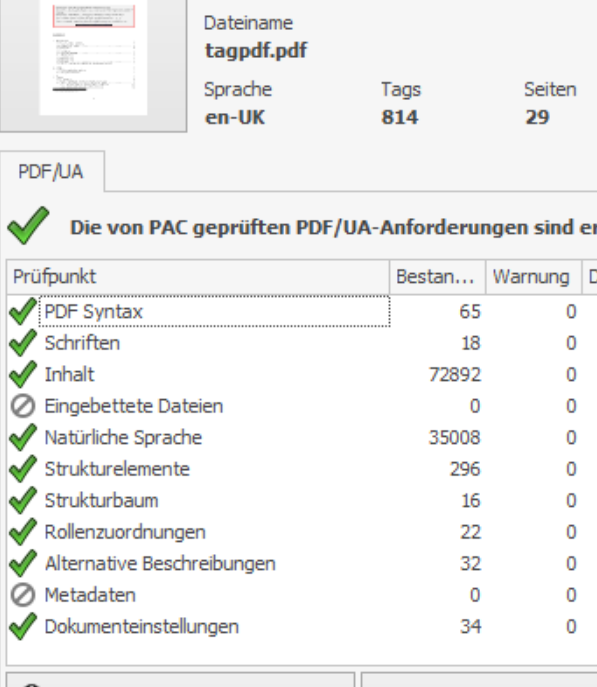
\includegraphics{pac3}
\tagmcend\tagstructend

\subsection{Changes in version 0.61}
\begin{itemize}
\item \TagP^internal code adaptions to expl3 changes.\Pmeti
\item \TagP^dropped the compresslevel key  -- probably not needed\Pmeti
\end{itemize}

\section{Setup}

\minisec{Activation needed!}
\TagP^When the package is loaded it will -- apart from loading more packages and defining a lot of things -- not do anything. You will have to activate it with \verb+\tagpdfsetup+, see below. (At least that's the theory, I'm not quite sure, if really the tests are done always as planed\ldots.)
\TagPend


\subsection{Modes and package options}

\TagP^The package has two different modes: The \textbf{generic mode} works (in theory, currently only with pdftex and luatex) probably with all engines, the \textbf{lua mode} only with luatex. The differences between both modes  will be described later. The mode can be set with package options:

\DescribeKey{luamode}

\TagP This is the default mode. It will use the generic mode if the document is processed with pdflatex and the lua mode with lualatex.

\DescribeKey{genericmode}

\TagP This will force the generic mode for all engines. \TagPend




\subsection{Setup and activation}\label{ssec:setup}

\TagP^The following command setups the general behaviour of the package. The command should be normally used only in the preamble (for a few keys it could also make sense to change them in the document).


\DescribeMacro\tagpdfsetup{<key-val-list>}


\TagP The key-val list understands the following keys:\TagPend
\begin{description}
\item[\PrintKeyName{activate-all}]
 \TagP^Boolean, initially false. Activates everything, that's normally the sensible thing to do.\Pmeti
\item[\PrintKeyName{activate-mc}]
 \TagP^Boolean, initially false. Activates the code related to marked content.\Pmeti
\item[\PrintKeyName{activate-struct}]
 \TagP^Boolean, initially false. Activates the code related to structures. Should be used only if \PrintKeyName{activate-mc} has been used too.\Pmeti
\item[\PrintKeyName{activate-tree}]
\TagP^ Boolean, initially false. Activates the code related to trees. Should be used only if the two other keys has been used too.\Pmeti
\item[\PrintKeyName{add-new-tag}]
 \TagP^Allows to define new tag names, see section \ref{sec:new-tag} for a description.\Pmeti
\item[\PrintKeyName{check-tags}]
 \TagP^Boolean, initially true. Activates some safety checks (but doesn't do very much currently. It will perhaps be merged with the log-level key).\Pmeti
\item[\PrintKeyName{inputencoding}]
 \TagP^Some keys convert their value and so need to know the encoding of the file. The default encoding is utf8.  When using pdflatex you can switch to another encoding with this key. The value should be one of names allowed by \texttt{l3str}. There is no checking that the name is valid (I don't think that it sensible to use something else than utf8).
 \Pmeti
\item[\PrintKeyName{interwordspace}]
 \TagP^Choice key, possible values are \PrintKeyName{true}/""\PrintKeyName{on} and \PrintKeyName{false}/\PrintKeyName{off}. The key activates/deactivates the insertion of space glyphs, see section~\ref{sec:spacechars}. In the luamode it only works if at least \PrintKeyName{activate-mc} has been used.\Pmeti
\item[\PrintKeyName{log}]
 \TagP^Choice key, possible values \PrintKeyName{none}, \PrintKeyName{v}, \PrintKeyName{vv}, \PrintKeyName{vvv},  \PrintKeyName{all}.  Setups the log level.  Changing the value affects currently mostly the luamode: \enquote{higher} values gives more messages in the log. The current levels and messages have been setup in a quite ad-hoc manner and will need improvement.\Pmeti
\item[\PrintKeyName{newattribute}]
 \TagP^This key takes two arguments and declares an attribute. See \ref{sec:attributes}.\Pmeti
\item[\PrintKeyName{show-spaces}]
\TagP^Boolean.\marginnote{luamode} That's a debug option, it helps to see where space glyph will be inserted if \PrintKeyName{interwordspace} is activated.\Pmeti
\item[\PrintKeyName{tabsorder}]
 \TagP^Choice key, possible values are \PrintKeyName{row}, \PrintKeyName{column}, \PrintKeyName{structure}, \PrintKeyName{none}.  This decides if a \verb+/Tabs+ value is written to the dictionary of the page objects. Not really needed for tagging itself, but one of the things you probably need for accessibility checks. So I added it. Currently the tabsorder is the same for all pages. Perhaps this should be changed \ldots.\Pmeti
\item[\PrintKeyName{tagunmarked}]
 \TagP^Boolean,\marginnote{luamode} initially true. When this boolean is true, the lua code will try to mark everything that has not been marked yet as an artifact. The benefit is that one doesn't have to mark up every deco rule oneself. The danger is that it perhaps marks things that shouldn't be marked -- it hasn't been tested yet with complicated documents containing annotations etc. See also section~\ref{sec:lazy} for a discussion about automatic tagging.\Pmeti
\item[\PrintKeyName{uncompress}]
 \TagP^Sets both the pdf compresslevel and the pdf objcompresslevel to 0 and so allows to inspect the pdf.\Pmeti


\end{description}


\section{Tagging}

\TagP^pdf is a page orientated graphic format. It simply puts ink and glyphs at various coordinates on a page. A simple stream of a page can look like this\footnote{The appendix contains some remarks about the syntax of a pdf file}:
\TagPend

\tagstructbegin{tag=Code}\tagmcbegin{tag=Code}
\begin{lstlisting}[columns=fixed]
stream
   BT
   /F27 14.3462 Tf                 %select font
   89.291 746.742 Td               %move point
   [(1)-574(Intro)-32(duction)]TJ  %print text
   /F24 10.9091 Tf                 %select font
    0 -24.35 Td                    %move point
    [(Let's)-331(start)]TJ         %print text
    205.635 -605.688 Td            %move point
    [(1)]TJ                        %print text
   ET
endstream
\end{lstlisting}
\tagmcend\tagstructend

\TagP^From this stream one can extract the characters and their placement on the page but not their semantic meaning  (the first line is actually a section heading, the last the page number). And while in the example the order is correct there is actually no guaranty that the stream contains the text in the order it should be read.

\TagP Tagging means to enrich the pdf with information about the \emph{semantic} meaning and the \emph{reading order}. (Tagging can do more, one can also store all sorts of layout information like font properties and indentation with tags. But as I already wrote this package concentrates on the part of tagging that is needed to improve accessibility.)\TagPend




\subsection{Three tasks}
\TagP^To tag a pdf three tasks must be  carried out:\TagPend

\begin{enumerate}
\item
  \TagP^\textbf{The mark-content-task}:\marginnote{mc-task} The document must add \enquote{labels} to the page stream which allows to identify and reference the various chunks of text and other content.  This is the most difficult part of tagging -- both for the document writer but also for the package code. At first there can be quite many chunks as every one is a leaf node of the structure and so often a rather small unit.  At second the chunks must be defined page-wise -- and this is not easy when you don't know where the page breaks are. Also in a standard document a lot text is created automatically, e.g. the toc, references, citations, list numbers etc and it is not always easy to mark them correctly.\Pmeti

\item
  \TagP^\textbf{The structure-task}:\marginnote{struct-task}  The document must declare the structure. This means marking the start and end of semantically connected portions of the document (correctly nested as a tree). This too means some work for the document writer, but less than for the mc-task: at first quite often the mc-task and the structure-task can be combined, e.g. when you mark up a list number or a tabular cell or a section header; at second one doesn't have to worry about page breaks so quite often one can patch standard environments to declare the structure. On the other side a number of structures end in \LaTeX\ only implicitly -- e.g. an item ends at the next item, so getting the pdf structure right still means that additional mark up must be added.
  \Pmeti

\item
 \TagP^\textbf{The tree management}:\marginnote{tree-task} At last the structure must be written into the pdf. For every structure an object of type \texttt{StructElem} must be  created and flushed with keys for the parents and the kids. A parenttree must be created to get a reference from the mc-chunks to the parent structure. A rolemap must be written. And a number of dictionary entries. All this is hopefully done automatically and correctly by the package \ldots.
 \Pmeti
\end{enumerate}


\begin{figure}[t!]
\begin{tcolorbox}

\minisec{Page stream with marked content}

\tagstructbegin{tag=Figure,alttext={Illustration of page stream with marked content}}%
\tagmcbegin{tag=Figure}%
\begin{tikzpicture}[baseline=(a.north),node distance=2pt,remember picture]
\node(start){\ldots~\ldots~\ldots};
\node[draw,base right = of start](a) {mc-chunk 1};
\node[draw,base right = of a](b) {mc-chunk 2};
\node[draw,base right = of b](c) {mc-chunk 3};
\node[draw,base right = of c](d) {mc-chunk 3};
\node[base right = of d] {\ldots~\ldots};
\end{tikzpicture}
\tagmcend\tagstructend


\minisec{Structure}

\newlength\ydistance\setlength\ydistance{-0.8cm}
\tagstructbegin{tag=Figure,alttext={Illustration of structure}}%
\tagmcbegin{tag=Figure}%
\begin{tikzpicture}[remember picture,baseline=(root.north)]

\node[draw,anchor=base west] (root) at (0,0) {Sect (start section)};
\node[draw,anchor=base west] at (0.3,\ydistance) {H (header section)};
\node[draw,anchor=base west](aref) at (0.6,2\ydistance){mc-chunk 1};
\node[draw,anchor=base west](bref) at (0.6,3\ydistance){mc-chunk 2};
\node[draw,anchor=base west] at (0.3,4\ydistance){/H (end header)};
\node[draw,anchor=base west] at (0.3,5\ydistance){P (start paragraph)};
\node[draw,anchor=base west](cref) at (0.6,6\ydistance){mc-chunk 3};
\node[draw,anchor=base west](dref) at (0.6,7\ydistance){mc-chunk 4};
\node[draw,anchor=base west] at (0.3,8\ydistance){/P (end paragraph)};
\node[draw,anchor=base west] at (0,9\ydistance){/Sect (end section)};
\end{tikzpicture}

\begin{tikzpicture}[remember picture, overlay]
\draw[->,red](aref)-|(a);
\draw[->,red](bref)-|(b);
\draw[->,red](cref)-|(c);
\draw[->,red](dref)-|(d);

\end{tikzpicture}
\tagmcend\tagstructend
\end{tcolorbox}
\tagstructbegin{tag=Caption}\tagmcbegin{tag=Caption}
\caption{Schematical description of the relation between marked content in the page stream and the structure}
\tagmcend\tagstructend

\end{figure}

\subsection{Task 1: Marking the chunks: the mark-content-step}

\TagP^To be able to refer to parts of the text in the structure, the text in the page stream must get \enquote{labels}. In the pdf reference they are called \enquote{marked content}. The three main variants needed here are:\TagPend

\begin{description}
\item[Artifacts] \TagP^They are marked with of a pair of keywords, \texttt{BMC} and \texttt{EMC} which surrounds the text. \texttt{BMC} has a single prefix argument, the fix tag name \texttt{/Artifact}. Artifacts should be used for irrelevant text and page content that should be ignored in the structure. Sadly it is often not possible to leave such text simply unmarked -- the accessibility tests in Acrobat and other validators complain.\TagPend

\tagstructbegin{tag=Code}\tagmcbegin{tag=Code}
\begin{lstlisting}
/Artifact BMC
 text to be marked
/EMC
\end{lstlisting}
\tagmcend\tagstructend\meti



\item[Artifacts with a type] \TagP^They are marked with of a pair of keywords, \texttt{BDC} and \texttt{EMC} which surrounds the text. \texttt{BDC} has two arguments: again the tag name \texttt{/Artifact} and a following dictionary which allows to specify the suppressed info. Text in header and footer can e.g. be declared as pagination like this:\TagPend

\tagstructbegin{tag=Code}\tagmcbegin{tag=Code}
\begin{lstlisting}
/Artifact <</Type /Pagination>> BDC
 text to be marked
/EMC
\end{lstlisting}
\tagmcend\tagstructend\meti


\item[Content]  \TagP^Content is marked also with of a pair of keywords, \texttt{BDC} and \texttt{EMC}. The first argument of \texttt{BDC} is a tag name which describes the structural type of the text\footnote{There is quite some redundancy in the specification here. The structural type is also set in the structure tree. One wonders if it isn't enough to use  always \texttt{/SPAN} here.}
    Examples are \texttt{/P} (paragraph), \texttt{/H2} (header), \texttt{/TD} (table cell). The reference mentions a number of standard types but it is possible to add more or to use different names.

\TagP In the second argument of \texttt{BDC} -- in the property dictionary -- more data can be stored. \emph{Required} is an \texttt{/MCID}-key which takes an integer as a value:\TagPend

\tagstructbegin{tag=Code}\tagmcbegin{tag=Code}
\begin{lstlisting}
/H <</MCID 3>> BDC
 text to be marked
/EMC
\end{lstlisting}
\tagmcend\tagstructend

\TagP^This integer is used to identify the chunk when building the structure tree. The chunks are numbered by page starting with 0. As the numbers are also used as an index in an array they shouldn't be \enquote{holes} in the numbering system
%\footnote{
(It is perhaps possible to handle a numbering scheme not starting by 0 and having holes, but it will enlarge the pdf as one would need dummy objects.).

\TagP It is possible to add more entries to the property dictionary, e.g. a title, alternative text or a local language setting.\Pmeti
\end{description}


\TagP^The needed markers can be added with low level code e.g. like this (in pdftex syntax):\TagPend

\tagstructbegin{tag=Code}\tagmcbegin{tag=Code}
\begin{lstlisting}
\pdfliteral page {/H <</MCID 3>> BDC}%
 text to be marked
\pdfliteral page {EMC}%
\end{lstlisting}
\tagmcend\tagstructend

\TagP^This sounds easy. But there are quite a number of traps.\TagPend

\begin{enumerate}[beginpenalty=10000]
  \item \TagP^Pdf is a page oriented format. And this means that the start \texttt{BDC}/\texttt{BMC}  and the corresponding end \texttt{EMC} must be on the same page.
  So marking e.g. a section title like in the following example won't always work as the literal before the section could end on the previous page:\TagPend

\tagstructbegin{tag=Code}\tagmcbegin{tag=Code}
\begin{lstlisting}
\pdfliteral page {/H <</MCID 3>> BDC} %problem: possible pagebreak here
 \section{mysection}
\pdfliteral page {EMC}%
\end{lstlisting}
\tagmcend\tagstructend

  \TagP^Using the literals \emph{inside} the section argument is better, but then one has to take care that they don't wander into the header and the toc.\Pmeti

  \item
  \TagP^Literals are \enquote{whatsits} nodes and can change spacing, page and line breaking. The literal \emph{behind} the section in the previous example could e.g. lead to a lonely section title at the end of the page.\Pmeti

  \item
   \TagP^The \texttt{/MCID} numbers must be unique on a page. So you can't use the literal in a saved box that you reuse in various places. This is e.\,g. a problem with \texttt{longtable} as it saves the table header and footer in a box.\Pmeti

  \item
  \TagP^The  \texttt{/MCID}-chunks are leaf nodes in the structure tree, so they shouldn't be nested.\Pmeti

  \item
  \TagP^Often text in a document is created automatically or moved around: entries in the table of contents, index, bibliography and more. To mark these text chunks correctly one has to analyze the code creating such content to find suitable places to inject the literals.\Pmeti

  \item
  \TagP^The literals are inserted directly and not at shipout. This means that due to the asynchronous page breaking of \TeX\ the MCID-number can be wrong even if the counter is reset at every page (this package uses in generic mode a label-ref-system to get around this problem. This sadly means that three compilations are needed until everything has settled down).\Pmeti

  \item
  \TagP^There exist environments which process their content more than once -- examples are \texttt{align} and \texttt{tabularx}.
       So one has to check for doublettes and holes in the counting system.\Pmeti


  \item
  \TagP^Pdf is a page oriented format. And this means that the start and the end marker must be on the same page \ldots\ \emph{so what to do with normal paragraphs that split over pages??}. This question will be discussed in subsection~\ref{sec:splitpara}.\Pmeti
\end{enumerate}

\subsubsection{Generic mode versus lua mode in the mc-task}

\TagP^While in generic mode the commands insert the literals directly and so have all the problems described above the lua mode works quite differently: The tagging commands don't insert literals but set some \emph{attributes} which are attached to all the following nodes. When the page is shipped out some lua code is called which wanders through the shipout box and injects the literals at the places where the attributes changes.

\TagP This means that quite a number of problems mentioned above are not relevant for the lua mode:\TagPend

\begin{enumerate}
\item \TagP^Pagebreaks between start and end of the marker are \emph{not} a problem. So you can mark a complete paragraph. If a pagebreak occur directly after an start marker or before an end marker this can lead to empty chunks in the pdf and so bloat up pdf a bit, but this is imho not really a problem (compared to the size increase by the rest of the tagging).\Pmeti
\item \TagP^The commands don't insert literals directly and so affect line and page breaking much less.\Pmeti
\item \TagP^The numbering of the MCID are done at shipout, so no label/ref system is needed.\Pmeti
\item \TagP^The code can do some marking automatically. Currently everything that has not been marked up by the document is marked as artifact.\Pmeti
\end{enumerate}

\subsubsection{Commands to mark content and chunks}

\TagP^It\marginnote{Generic mode only} is vital that the end command is executed on the same page as the begin command. So think carefully how to place them.
For strategies how to handle paragraphs that split over pages see subsection~\ref{sec:splitpara}.\TagPend

\ExplSyntaxOn
\DescribeMacro\tagmcbegin{<key-val-list>}
\DescribeMacro\uftag_mc_begin:n{<key-val-list>}
\ExplSyntaxOff

\TagP^These commands insert the begin of the marked content code in the pdf. They don't start a paragraph. \emph{They don't start a group}. The user command additionally issues an \verb+\ignorespaces+ to suppress spaces after itself.
Such markers should not be nested. The command will warn you if this happens.


\TagP The key-val list understands the following keys:\TagPend
\begin{description}
  \item[\PrintKeyName{tag}]
  \TagP^This is required, unless you use the \PrintKeyName{artifact} key. The value of the key is normally one of the standard type listed in section \ref{sec:new-tag} (without a slash at the begin, this is added by the code). It is possible to setup new tags, see the same section. The value of the key is expanded, so it can be a command. The expansion is passed unchanged to the pdf, so it should with a starting slash give a valid pdf name  (some ascii with numbers like \texttt{H4} is fine).\Pmeti

  \item[\PrintKeyName{artifact}]
  \TagP^This will setup the marked content as an artifact. The key should be used for content that should be ignored. The key can take one of the values \PrintKeyName{pagination}, \PrintKeyName{layout},  \PrintKeyName{page},  \PrintKeyName{background} and \PrintKeyName{notype} (this is the default). Text in the header and footer should be marked with \PrintKeyName{artifact=pagination}.

  \TagP    It is not quite clear if rules and other decorative graphical objects needs to be marked up as artifacts. Acrobat seems not to mind if not, but PAC~3 complained.

  \TagP    The validators complain if some text is not marked up, but it is not quite clear if this is a serious problem.

  \TagP    The\marginnote{lua mode only} lua mode will mark up everything unmarked as \texttt{artifact=notype}. You can suppress this behaviour by setting the tagpdfsetup key \texttt{tagunmarked} to false. See section \ref{ssec:setup}.\Pmeti

  \item[\PrintKeyName{stash}]
   \TagP^Normally marked content will be stored in the \enquote{current} structure. This may not be what you want. As an example you may perhaps want to put a marginnote behind or before the paragraph it is in the tex-code. With this boolean key the content is marked but not stored in the kid-key of the current structure.\Pmeti

  \item[\PrintKeyName{label}]
  \TagP^This key sets a label by which you can call the marked content later in another structure (if it has been stashed with the previous key). Internally the label name will start with \texttt{tagpdf-}.\Pmeti

  \item[\PrintKeyName{alttext}]
   \TagP^This key inserts an \texttt{/Alt} value in the property dictionary of the BDC operator. See section~\ref{sec:alttext}. The value is handled as verbatim string, commands are not expanded.\Pmeti
  \item[\PrintKeyName{alttext-o}]
  \TagP^This key inserts an \texttt{/Alt} value in the property dictionary of the BDC operator. See section~\ref{sec:alttext}. The value is handled as verbatim string like the key \PrintKeyName{alttext} but expanded once (the \texttt{o} refers to the \texttt{o} type in expl3).
  That means that you can do something like this: \TagPend
  \tagstructbegin{tag=Code}\tagmcbegin{tag=Code}
      \begin{lstlisting}
      \newcommand\myalttext{\frac{a}{b}}
      \tagmcbegin{tag=P,alttext-o=\myalttext}
      \end{lstlisting}
  \tagmcend\tagstructend

  \TagP^    and it will insert \verb+\frac{a}{b}+  (hex encoded) in the pdf.\Pmeti

  \item[\PrintKeyName{actualtext}]
  \TagP^This key inserts an \texttt{/ActualText} value in the property dictionary of the BDC operator. See section~\ref{sec:alttext}. The value is handled as verbatim string, commands are not expanded.\Pmeti


  \item[\PrintKeyName{actualtext-o}]
  \TagP^This key inserts an \texttt{/ActualText} value in the property dictionary of the BDC operator. See section~\ref{sec:alttext}. The value is handled as verbatim string like the key \PrintKeyName{actualtext} but expanded once (the \texttt{o} refers to the \texttt{o} type in expl3). That means that you can do something like this:\TagPend

\tagstructbegin{tag=Code}\tagmcbegin{tag=Code}
      \begin{lstlisting}
      \newcommand\myactualtext{X}
      \tagmcbegin{tag=P,alttext-o=\myactualtext}
      \end{lstlisting}
 \tagmcend\tagstructend


 \TagP^and it will insert \verb+X+ (hex encoded)  in the pdf.\Pmeti

  \item[\PrintKeyName{raw}]
  \TagP^This key allows you to add more entries to the properties dictionary. The value must be correct, low-level pdf. E.g. \verb+raw=/Alt (Hello)+ will insert an alternative Text.\Pmeti
\end{description}


\ExplSyntaxOn
\DescribeMacro\tagmcend
\DescribeMacro\uftag_mc_end:
\ExplSyntaxOff

\TagP^These commands insert the end code of the marked content. They don't end a group and in generic mode it doesn't matter if they are in another group as the starting commands. The user command also issues at first an \verb+\unskip+. In generic mode both commands check if there has been a begin marker and issue a warning if not. In luamode it is often possible to omit the command, as the effect of the begin command ends with the current group or with a new \verb+\tagmcbegin+ anyway.\TagPend

\begin{tcolorbox}
\minisec{About nesting mc-commands}
\TagP^\textbf{Attention!}\marginnote{luamode} As mentioned above in luamode it is often possible to omit the \verb+\tagmcend+ command. This basically means that mc-chunks can be nested.  But be aware that this can have surprising side effects on the order in the structure.

\TagP Consider a code like this:\TagPend

\tagstructbegin{tag=Code}\tagmcbegin{tag=Code}
\begin{lstlisting}
\tagmcbegin{tag=P} Block 1 {\tagmcbegin{tag=P Block 2}} Block 3 \tagmcend
\end{lstlisting}
\tagmcend\tagstructend

\TagP^Block 3 will here get the same id number as Block 1 and be stored in the structure \emph{before} Block 2. The pdf will record the chunks in the order \texttt{Block 1 -- Block 3 -- Block 2}.
\TagPend
\end{tcolorbox}

\ExplSyntaxOn
\DescribeMacro\tagmcuse{<label name>}
\DescribeMacro\uftag_mc_use:n {<label name>}
\ExplSyntaxOff

\TagP^These commands allow you to record a marked content that you stashed away into the current structure. Be aware that a marked content can be used only once -- the command will warn you if you try to use it a second time.\TagPend

\ExplSyntaxOn
\DescribeMacro\tagmcifinTF{<true code>}{<false>}
\DescribeMacro\uftag_mc_if_in:TF{<true code>}{<false>}
\ExplSyntaxOff

\TagP^These commands check if a marked content is currently open and allows you to e.g. add the end marker if yes.

\TagP In \emph{generic mode}, where marked content command shouldn't be nested, it works with a global boolean.

\TagP In \emph{lua mode} it tests if the mc-attribute is currently unset. You can't test the nesting level with it!\TagPend

\ExplSyntaxOn
\DescribeMacro\tagpdfget{<key word>}
\DescribeMacro\uftag_get:n{<key word>}
\ExplSyntaxOff

\TagP^These commands give back some variables. Currently the only working key word is \verb+mc\_tag+.\TagPend.

\subsubsection{Tips}

\begin{itemize}
\item \TagP^Mark commands inside floats should work fine (but need perhaps some compilation rounds in generic mode).\Pmeti
\item \TagP^In case you want to use it inside a \verb+\savebox+ (or some command that saves the text internally in a box): If the box is used directly, there is probably no problem. If the use is later, stash the marked content and add the needed \verb+\tagmcuse+ directly  before oder after the box when you use it.\Pmeti
\item \TagP^Don't use a saved box with markers twice.\Pmeti
\item \TagP^If boxes are unboxed you will have to analyze the pdf to check if everything is ok.\Pmeti
\item \TagP^If you use complicated structures and commands (breakable boxes like the one from tcolorbox, multicol, many footnotes) you will have to check the pdf.\Pmeti
 \end{itemize}


\begin{figure}
\tagstructbegin{tag=Figure,alttext={Illustration of link annotation structure}}\tagmcbegin{tag=Figure}
% needs 
%\usepackage{listings}
%\usepackage{tikz}
%\usetikzlibrary{fit,tikzmark}
%\usetikzlibrary{arrows.meta}
\lstset{basicstyle=\ttfamily,
        columns=flexible,
        escapechar=*,
        morecomment=[l]{\%},keepspaces=true,
        commentstyle=\color{green!50!black}\bfseries}
\tikzset{
  balloon/.style={
    draw,
    fill=blue!20,
    opacity=0.4,
    inner xsep=4pt,inner ysep=2pt,
    rounded corners=2pt,
    %minimum height=15pt
  },
  ref/.style={
  very thick, -Latex,red
  },
  iref/.style={
  thick,dashed, -Latex,red
  }
}
\NewDocumentCommand\balloon{m}{%
\node[fit={(pic cs:#1-first) (pic cs:#1-end)
([yshift=7pt]pic cs:#1-end)},balloon](#1){};}
\begin{tikzpicture}[overlay,remember picture]
\balloon{link}
\balloon{structparent}
\balloon{OBJR}
\balloon{linkref}
\balloon{structelem}
\balloon{kid}
\balloon{pnum}
\balloon{pref}
\draw[ref] (linkref)--(link);
\draw[ref] (link)--(structparent.170);
\draw[ref] (structparent.190)--(pnum);
\draw[ref] (pnum)--(pref);
\draw[ref] (pref)--(structelem);
\draw[ref] (structelem)--(kid);
\draw[ref] (kid)--(OBJR);
\draw[ref] (OBJR)--(linkref);
\end{tikzpicture}
\begin{lstlisting}[name=OBJR]
*\tikzmark{link-first}*18 0 obj*\tikzmark{link-end}*   %Link Object
<< /Type /Annot /Subtype/Link
   /Rect [ 196.109 494.573 399.167 506.831 ]
*\tikzmark{structparent-first}*/StructParent 16 *\tikzmark{structparent-end}*
 /A<</Type/Action /S/URI /URI(https://github.com/u-fischer/tagpdf)>>
 >>
endobj

*\tikzmark{OBJR-first}*19 0 obj*\tikzmark{OBJR-end}*   %Object reference (OBJR)
<</Type /OBJR /Obj *\tikzmark{linkref-first}*18 0 R*\tikzmark{linkref-end}* >>
endobj

*\tikzmark{structelem-first}*17 0 obj*\tikzmark{structelem-end}*   %Structure Element
<< /Type /StructElem /S /Link /P 11 0 R
/K [<</Type /MCR /Pg 8 0 R /MCID 6>> *\tikzmark{kid-first}*19 0 R*\tikzmark{kid-end}* ]>>
endobj};

5 0 obj   %Parenttree
<< /Nums
[... *\tikzmark{pnum-first}*16*\tikzmark{pnum-end}*     *\tikzmark{pref-first}*17 0 R*\tikzmark{pref-end}* ...] >>
endobj
\end{lstlisting}

\tagmcend\tagstructend
\tagstructbegin{tag=Caption}\tagmcbegin{tag=Caption}
\caption{Structure needed for a link annotation}\label{fig:linkannot}
\tagmcend\tagstructend
\end{figure}

\subsubsection{Links}

\TagP^Link annotations (like all PDF annotations) are associated with a geometric region of the page rather than with a particular object in its content stream. Any connection between the link and the content is based solely on visual appearance rather than on an explicitly specified association.\TagPend

\TagP^To connect such a link with the underlying text a specific structure has to be added, see \ref{fig:linkannot}. When using the low-level commands to create a link, this structure can be created by adding an entry to the attr argument of the startlink command, and by by adding a command of the tagpdf package after the endlink command, as show in the following listing:\TagPend

\tagstructbegin{tag=Code}\tagmcbegin{tag=Code}
\begin{lstlisting}
\pdfextension startlink
    attr
     {
     /StructParent \int_use:N\c@g__uftag_parenttree_obj_int %<----
     }
    user {
          /Subtype/Link
          /A
           <<
            /Type/Action
            /S/URI
            /URI(http://www.dante.de)
           >>
         }
    This is a link.
\pdfextension endlink
\__uftag_struct_finish_link: %<----
\end{lstlisting}
\tagmcend\tagstructend

\TagP^The question is here is how to add this to the hyperref commands without doing a lot patching? This had lead to a new project which tries to move some definitions for links to the \LaTeX-kernel so that package likes hyperref and tagpdf can coexist and both add their code to links at the same time.\TagPend

\subsubsection{Math}

\TagP^Math is a problem. I have seen an example where \emph{every single symbol} has been marked up with tags from MathML along with an \texttt{/ActualText} entry and an entry with alternate text which describes how to read the symbol.
The pdf then looked like this\TagPend

\tagstructbegin{tag=Code}\tagmcbegin{tag=Code}
\begin{lstlisting}
/mn <</MCID 6 /ActualText<FEFF0034>/Alt(  : open bracket: four )>>BDC
...
/mn <</MCID 7 /ActualText<FEFF0033>/Alt(  third s  )>>BDC
...
/mo <</MCID 8 /ActualText<FEFF2062>/Alt(  times  )>>BDC
\end{lstlisting}
\tagmcend\tagstructend


\TagP^If this is really the way to go one would need some script to add the mark-up as doing it manually is too much work and would make the source unreadable -- at least with pdflatex and the generic mode. In lua mode is it probably possible to hook into the \texttt{mlist\_to\_hlist} callback and add marker automatically.\TagPend

\TagP^But I'm not sure that this is the best way to do math. It looks rather odd that a document should have to tell a screen reader in such detail how to read an equation. It would be much more efficient, sensible and flexible if a complete representation of the equation in mathML could be stored in the pdf and the task how to read this aloud delegated to the screen reader. More investigations are needed here.\TagPend

\TagP^See also section~\ref{sec:alttext} for some more remarks and tests.\TagPend

\subsubsection{Split paragraphs}\label{sec:splitpara}

\TagP^A\marginnote{Generic mode only} problem are paragraphs with page breaks.  As already mentioned the end marker \texttt{EMC} must be added on the same page as the begin marker. But it is in pdflatex \emph{very} difficult to inject something at the page break automatically. One can manipulate the shipout box to some extend in the output routine, but this is not easy and it gets even more difficult if inserts like footnotes and floats are involved: the end of the paragraph is then somewhere in the middle of the box.

\TagP So with pdflatex in generic mode one currently has to do the splitting manually.

\TagP The example \texttt{mc-manual-para-split} demonstrates how this can be done. The general idea is to use \verb+\vadjust+ in the right place:\TagPend

\tagstructbegin{tag=Code}\tagmcbegin{tag=Code}
\begin{lstlisting}
\tagmcbegin{tag=P}
...
fringilla, ligula wisi commodo felis, ut adipiscing felis dui in
enim. Suspendisse malesuada ultrices ante.% page break
\vadjust{\tagmcend\pagebreak\tagmcbegin{tag=P}}
Pellentesque scelerisque
...
sit amet, lacus.\tagmcend
\end{lstlisting}
\tagmcend\tagstructend



\subsection{Task 2: Marking the structure}
\TagP^The structure is represented in the pdf with a number of objects of type \texttt{StructElem} which build a tree: each of this objects points back to its parent and normally has a number of kid elements, which are either again structure elements or -- as leafs of the tree -- the marked contents chunks marked up with the \verb+tagmc+-commands. The root of the tree is the \texttt{StructTreeRoot}.\TagPend

\subsubsection{Structure types}
\TagP^The tree should reflect the \emph{semantic} meaning of the text. That means that the text should be marked as section, list, table head, table cell and so on. A number of standard structure types is predefined, see section \ref{sec:new-tag} but it is allowed to create more. If you want to use types of your own you must declare them. E.g. this declares two new types \texttt{TAB} and {FIG} and base them on \texttt{P}:\TagPend

\tagstructbegin{tag=Code}\tagmcbegin{tag=Code}
\begin{lstlisting}
\tagpdfsetup{
  add-new-tag = TAB/P,
  add-new-tag = FIG/P,
            }
\end{lstlisting}
\tagmcend\tagstructend

\subsubsection{Sectioning}
\TagP^The sectioning units can be structured in two ways: a flat, html-like and a more xml-like version.
The flat version creates a structure like this:\TagPend

\tagstructbegin{tag=Code}\tagmcbegin{tag=Code}
\begin{lstlisting}
<H1>section header</H1>
<P> text</P>
<H2>subsection header</H2>
...
\end{lstlisting}
\tagmcend\tagstructend

\TagP^So here the headers are marked according their level with \texttt{H1}, \texttt{H2}, etc.

\TagP In the xml-like tree the complete text of a sectioning unit is surrounded with the \texttt{Sect} tag, and all headers with the tag \texttt{H}. Here the nesting defines the level of a sectioning header.\TagPend

\tagstructbegin{tag=Code}\tagmcbegin{tag=Code}
\begin{lstlisting}
<Sect>
 <H>section header</H>
 <P> text</p>
 <Sect>
   <H>subsection header</H>
   ...
 </Sect>
</Sect>
\end{lstlisting}
\tagmcend\tagstructend

\TagP^The flat version is more \LaTeX-like and it is rather straightforward to patch \verb+\chapter+, \verb+\section+ and so on to insert the appropriates \texttt{H\ldots} start and end markers. The xml-like tree is more difficult to automate. If such a tree is wanted I would recommend to use -- like the context format -- explizit commands to start and end a sectioning unit.
\TagPend

\subsubsection{Commands to define the structure}
\TagP^The following commands can be used to define the tree structure:

\ExplSyntaxOn
\DescribeMacro\tagstructbegin{key-val-list}
\DescribeMacro\uftag_struct_begin:n {key-val-list}
\ExplSyntaxOff

\TagP These commands start a new structure. They don't start a group. They set all their values globally.

\TagP The key-val list understands the following keys:\TagPend

\begin{description}
  \item[\PrintKeyName{tag}]
   \TagP^This is required. The value of the key is normally one of the standard type listed in section \ref{sec:new-tag}. It is possible to setup new tags/types, see the same section.\Pmeti

  \item[\PrintKeyName{stash}]
   \TagP^Normally a new structure inserts itself as a kid into the currently active structure. This key prohibits this. The structure is nevertheless from now on \enquote{the current active structure} and parent for following  marked content and structures.\Pmeti

  \item[\PrintKeyName{label}]
   \TagP^This key sets a label by which you can use the structure later in another structure. Internally the label name will start with \texttt{tagpdfstruct-}.\Pmeti


  \item[\PrintKeyName{alttext}]
   \TagP^This key inserts an \texttt{/Alt} value in the dictionary of structure object, see section~\ref{sec:alttext}. The value is handled as verbatim string and hex encoded.\Pmeti

  \item[\PrintKeyName{alttext-o}]
   \TagP^This key inserts an \texttt{/Alt} value in the dictionary of a structure object,  see section~\ref{sec:alttext}. The value is handled as verbatim string like the key \PrintKeyName{alttext} but expanded once (the \texttt{o} refers to the \texttt{o} type in expl3). That means that you can do something like this:\TagPend

   \tagstructbegin{tag=Code}\tagmcbegin{tag=Code}
      \begin{lstlisting}
      \newcommand\myalttext{\frac{a}{b}}
      \tagstructbegin{tag=P,alttext-o=\myalttext}
      \end{lstlisting}
   \tagmcend\tagstructend


   \TagP^   and it will insert \verb+\frac{a}{b}+  (hex encoded) in the pdf.\Pmeti


  \item[\PrintKeyName{actualtext}]
   \TagP^This key inserts an \texttt{/ActualText} value in the dictionary of structure object,  see section~\ref{sec:alttext}. The value is handled as verbatim string, commands are not expanded.\Pmeti

  \item[\PrintKeyName{actualtext-o}]
   \TagP^This key inserts an \texttt{/ActualText} value in the dictionary of structure object, see section~\ref{sec:alttext}. The value is handled as verbatim string like the key \PrintKeyName{actualtext} but expanded once (the \texttt{o} refers to the \texttt{o} type in expl3). That means that you can do something like this:\TagPend

   \tagstructbegin{tag=Code}\tagmcbegin{tag=Code}
      \begin{lstlisting}
      \newcommand\myactualtext{X}
      \tagstructbegin{tag=P,alttext-o=\myactualtext}
      \end{lstlisting}
   \tagmcend\tagstructend


   \TagP^and it will insert \verb+X+ (hex encoded)  in the pdf.\Pmeti

   \item[\PrintKeyName{attribute}]
    \TagP^This key takes as argument a comma list of attribute names (use braces to protect the commas from the external key-val parser) and allows to add one or more attribute dictionary entries in the structure object. As an example\TagPend
    \tagstructbegin{tag=Code}\tagmcbegin{tag=Code}
      \begin{lstlisting}
      \tagstructbegin{tag=TH,attribute= TH-row}
      \end{lstlisting}\tagmcend\tagstructend

    \TagP^See also section~\ref{sec:attributes}.\Pmeti

  \item[\PrintKeyName{attribute-class}]
   \TagP^This key takes as argument a comma list of attribute names (use braces to protect the commas from the external key-val parser) and allows to add one or more attribute classes to the structure object. As an example\TagPend

   \tagstructbegin{tag=Code}\tagmcbegin{tag=Code}
      \begin{lstlisting}
      \tagstructbegin{tag=TH,attribute-class= TH-row}
      \end{lstlisting}\tagmcend\tagstructend

  \TagP^See also section~\ref{sec:attributes}.\Pmeti

  \item[\PrintKeyName{title}]
  \TagP^This key allows to set the dictionary entry \texttt{/Title} in the structure object. The value is handled as verbatim string and hex encoded. Commands are not expanded.\Pmeti

  \item[\PrintKeyName{title-o}]
  \TagP^This key allows to set the dictionary entry \texttt{/Title} in the structure object.
  The value is expanded once and then handled as verbatim string like the \PrintKeyName{title} key.\Pmeti
\end{description}


\ExplSyntaxOn
\DescribeMacro\tagstructend
\DescribeMacro\uftag_struct_end:
\ExplSyntaxOff

\TagP^These commands end a structure. They don't end a group and it doesn't matter if they are in another group as the starting commands.\TagPend

\ExplSyntaxOn
\DescribeMacro\tagstructuse{<label>}
\DescribeMacro\uftag_struct_use:n {<label>}
\ExplSyntaxOff

\TagP^These commands insert a structure previously stashed away as kid into the currently active structure. A structure should be used only once, if the structure already has a parent you will get a warning.\TagPend

\subsubsection{Root structure}

\TagP^A document should have at least one structure which contains the whole document. A suitable tag is \texttt{Document} or \texttt{Article}. I'm considering to automatically inserting it.\TagPend

\subsubsection{Attributes and attribute classes}\label{sec:attributes}

\TagP^Structure Element can have so-called attributes. A single attribute is a dictionary%\footnote{
(or a stream but this is currently not supported by the package as I don't know an use-case)
with at least the required key \verb+/Owner+ which describes the scope the attribute applies too.
As an example here an attribute that can be attached to tabular header (type TH) and adds the info that the header is a column header:\TagPend

\tagstructbegin{tag=Code}\tagmcbegin{tag=Code}
\begin{lstlisting}
<</Owner /Table /Scope /Column>>
\end{lstlisting}
\tagmcend\tagstructend

\TagP^One or more such attributes can be attached to a structure element. It is also possible to store such an attribute under a symbolic name in a so-called \enquote{ClassedMap} and then to attach references to such classes to a structure.\TagPend

\TagP^To use such attributes you must at first declare it in \verb+\tagpdfsetup+ with the key \texttt{newattribute}. This key takes two argument, a name and the content of the attribute.
The name should be a sensible key name, the content a dictionary.
\TagPend

\tagstructbegin{tag=Code}\tagmcbegin{tag=Code}
\begin{lstlisting}
\tagpdfsetup
 {
  newattribute =
   {TH-col}{<</Owner /Table /Scope /Column>>},
  newattribute =
   {TH-row}{<</Owner /Table /Scope /Row>>},
  }
\end{lstlisting}
\tagmcend\tagstructend


\TagP^Attributes are only written to the pdf when used, so it is not a problem to predeclare a number of standard attributes.
\TagPend

\TagP^It is your responsability that the content of the dictionary is valid pdf and that the values are sensible!
\TagPend

\TagP^Attributes can then be used with the key \PrintKeyName{attribute} or \PrintKeyName{attribute-class} which both take a comma list of attribute names as argument:
%\footnote{That's not really a sensible example}:
\TagPend

\tagstructbegin{tag=Code}\tagmcbegin{tag=Code}
\begin{lstlisting}
\tagstructbegin{tag=TH,
 attribute-class= {TH-row,TH-col},
 attribute      = {TH-row,TH-col},
 }
\end{lstlisting}
\tagmcend\tagstructend


\subsection{Task 3: tree Management}
\TagP^When all the document content has been correctly marked and the data for the trees has been collected they must be flushed to the pdf. This is done automatically (if the package has been activated) with the following command in \verb+\AfterEndDocument+:\TagPend

\ExplSyntaxOn
\DescribeMacro\uftag_finish_structure:
\ExplSyntaxOff

\TagP^This will hopefully write all the needed objects and values to the pdf. (Beside the already mentioned  \texttt{StructTreeRoot} and \texttt{StructElem} objects, additionally a so-called \texttt{ParentTree} is needed which records the parents of all the marked contents bits, a \texttt{Rolemap}, perhaps a \texttt{ClassMap} and object for the attributes, and a few more values and dictionaries).\TagPend

\TagP^I'm not quite sure if this shouldn't be a really internal command.\TagPend


\subsection{A fully marked up document body}
\TagP^The following shows the marking needed for a section, a sentence and a list with two items. It is obvious that one wouldn't like to have to do this for real documents. If tagging should be usable, the commands must be hidden as much as possible inside suitable \LaTeX\ commands and enviroments.\TagPend

\tagstructbegin{tag=Code}\tagmcbegin{tag=Code}
\begin{lstlisting}
\begin{document}

\tagstructbegin{tag=Document}

 \tagstructbegin{tag=Sect}
  \tagstructbegin{tag=H}
   \tagmcbegin{tag=H} %avoid page break!
    \section{Section}
   \tagmcend
  \tagstructend
  \tagstructbegin{tag=P}
   \tagmcbegin{tag=P,raw=/Alt (x)}
    a paragraph\par x
   \tagmcend
  \tagstructend

 \tagstructbegin{tag=L} %List
  \tagstructbegin{tag=LI}
   \tagstructbegin{tag=Lbl}
    \tagmcbegin{tag=Lbl}
    1.
    \tagmcend
   \tagstructend
   \tagstructbegin{tag=LBody}
    \tagmcbegin{tag=P}
    List item body
    \tagmcend
   \tagstructend %lbody
  \tagstructend %Li

  \tagstructbegin{tag=LI}
   \tagstructbegin{tag=Lbl}
    \tagmcbegin{tag=Lbl}
    2.
    \tagmcend
   \tagstructend
   \tagstructbegin{tag=LBody}
    \tagmcbegin{tag=P}
    another List item body
    \tagmcend
   \tagstructend %lbody
  \tagstructend %Li
  \tagstructend %L

  \tagstructend  %Sect
\tagstructend   %Document
\end{document}
\end{lstlisting}
\tagmcend\tagstructend


\subsection{Lazy and automatic tagging}\label{sec:lazy}

\TagP^A number of features of pdf readers need a fully tagged pdf. As an example screen readers tend to ignore alternative text (see section~\ref{sec:alttext}) if the pdf is not fully tagged. Also reflowing a pdf only works for me (even if real space chars are in the pdf) if the pdf is fully tagged.\TagPend

\TagP^This means that even if you don't care about a proper structure you should try to add at least some minimal tagging. With pdflatex this is not easy due to the page break problem. But with lualatex you can use an \texttt{Document} structure and inside it rather large mc-chunks. This minimizes the needed work.\TagPend

\TagP^One could ask if in lua mode the code couldn't try to mark up unmarked parts e.g. as P-type chunks, like it marks them up as artifacts currently. Sadly this is not so easy, as it is quite difficult to reliably identify the structure and the place in the kids array where such chunks belongs too. I also don't think that it is really needed. It is not so difficult to define user macros which e.g. opens a structure and start an mc-chunk or which close an open mc-chunk before issuing the next \verb+\tagmcbegin+.
\TagPend


\section{Alternative text, ActualText and text-to-speech software}\label{sec:alttext}

\TagP^The pdf format allows to add alternative text through the  \PrintKeyName{/Alt} and the \PrintKeyName{/ActualText} key.
%\footnote{
There is also the \PrintKeyName{/E} key for acronyms but I will ignore it for now.
Both can be added either to the marked content in the page stream or to the object describing the structure.\TagPend

\TagP^The value of \PrintKeyName{/ActualText} (inserted by \texttt{tagpdf} with \PrintKeyName{actualtext}) is meant to replace single characters or rather small pieces of text. It can be used also without any tagging (e.g. with the package accsupp). If the pdf reader support this (adobe reader does, sumatra not) one can change with it how a piece of text is copied and pasted e.g. to split up a ligature.\TagPend

\TagP^\PrintKeyName{/Alt} (inserted by \texttt{tagpdf} with \PrintKeyName{alttext}) is a key to improve accessibility: with it one can add to a picture or something else an alternative text.\TagPend

\TagP^The file \texttt{ex-alt-actualtext.tex} shows some experiments I made with with both keys and text-to-speech software (the in-built of adobe and nvda).
To sum them up:\TagPend

\begin{itemize}
\item \TagP^The keys have an impact on text-to-speech software only if the document is fully tagged.\Pmeti
\item \TagP^\PrintKeyName{/ActualText} should be at best used around short pieces of marked content.\Pmeti
\item \TagP^\PrintKeyName{/Alt} is used at best with a structure -- this avoids problems with luatex where marked contents blocks can be split over pages.\Pmeti
\item \TagP^To some extend one can get a not so bad reading of math with the alternative text.\Pmeti
\end{itemize}






\section{Standard type and new tags}\label{sec:new-tag}

\TagP^The pdf reference mentions a number of standard types:
\ExplSyntaxOn
\clist_use:Nn \c__uftag_role_sttags_clist {,\c_space_tl}

\ExplSyntaxOff\TagPend

\TagP^Their meaning can be looked up in the pdf-reference \parencite{pdfreference}.\TagPend

\TagP^New tags can be defined in the setup command with the key \texttt{add-new-tag}. It takes a value consisting of two names separated by a slash. The first is the new name, the second a known (e.g. a standard) tag it should be mapped too. Example:\TagPend

\tagstructbegin{tag=Code}\tagmcbegin{tag=Code}
\Macro\tagpdfsetup{add-new-tag = section/H1}
\tagmcend\tagstructend



\section{\enquote{Real} space glyphs}\label{sec:spacechars}

\TagP^TeX uses only spaces (horizontal movements) to separate words. That means that a pdf reader has to use some heuristic when copying text or reflowing the text to decide if a space is meant as a word boundary or e.g. as a kerning. Accessible document should use real space glyphs (U+0032) from a font in such places.\TagPend

\TagP^With the key \PrintKeyName{interwordspace} you can activate such space glyphs.\TagPend

\TagP^With pdftex this will simply call the primitive \verb+\pdfinterwordspaceon+. pdftex will then insert at various places a char from a font called dummy-space. Attention! This means that at every space there are additional font switches in the pdf: from the current font to the dummy-space font and back again. This will make the pdf larger. As \verb+\pdfinterwordspaceon+ is a primitive function it can't be fine tuned or adapted. You can only turn it on and off and insert manually such a space glyph with \verb+\pdffakespace+.\TagPend

\TagP^With luatex (in luamode) interwordspace is implemented with a lua-function which is inserted in two callbacks and marks up the places where it seems sensible to inter a space glyph. Later in the process (when also the mc-markers are inserted) the space glyphs are injected -- the code will take the glyph from the current font if this has a space glyph or switch to the default latin modern font. The current code works reasonable well in normal text.\TagPend

\TagP^The key \PrintKeyName{show-spaces} will show lines at the places where in lua mode spaces are inserted and so can help you to find problematic places. For listings -- which have a quite specific handling of spaces -- you can find a suggestion in the example \texttt{ex-space-glyph-listings}.\TagPend

\TagP^\emph{Attention:} Even with real spaces copy\& pasting of code doesn't need to give the correct results: you get spaces but not necessarly the right number of spaces. The pdf viewers I tried all copied four real space glyphs as one space. I only got the four spaces with the export to text or xml in the AdobePro.\TagPend

\DescribeMacro\pdffakespace

\TagP^This is in pdftex a primitive. It inserts the dummy space glyph. \pkg{tagpdf} defines this command also for luatex -- attention if can perhaps insert break points.\TagPend



\section{Accessibility is not only tagging}

\TagP^A tagged pdf is needed for accessibility but this is not enough. As already mentioned there are more requirements:\TagPend

 \begin{itemize}
 \item \TagP^The language must be declared by adding a \texttt{/Lang xx-XX} to the pdf catalog or -- if the language changes for a part of the text to the structure or the marked content. Setting the document language can be rather easily done with existing packages or even directly with \verb+\pdfcatalog{/Lang (en-US)}+. For settings in marked content and structure I will have to add keys.\Pmeti
 \item \TagP^All characters must have an unicode representation or a suitable alternative text.
      With lualatex and open type (unicode) fonts this is normally not a problem. With pdflatex it could need\TagPend
      \tagstructbegin{tag=Code}\tagmcbegin{tag=Code}
      \begin{verbatim}
      \input{glyphtounicode}
      \pdfgentounicode=1
      \end{verbatim}
      \tagmcend\tagstructend

 \TagP^and perhaps some\verb+\pdfglyphtounicode+ commands.\Pmeti
 \item \TagP^Hard and soft hyphen must be distinct.\Pmeti
 \item \TagP^Spaces between words should be space glyphs and not only a horizontal movement. See section~\ref{sec:spacechars}.\Pmeti
 \item \TagP^Various small infos must be present in the catalog dictionary, info dictionary and the page dictionaries, e.g. metadata like title.\Pmeti
\end{itemize}
 \TagP^If suitable I will add code for this tasks to this packages. But some of them can also be done already with existing packages like hyperref, hyperxmp, pdfx.\TagPend



\section{To-do}
\begin{itemize}
\item \TagP^Add commands and keys to enable/disable the checks.\Pmeti
\item \TagP^Check/extend the code for language tags.\Pmeti
\item \TagP^Think about math.\Pmeti
\item \TagP^Think about Links/Annotations\Pmeti
\item \TagP^Keys for alternative and actualtext. How to define the input encoding? Like in Accsupp?\Pmeti
\item \TagP^Check twocolumn documents\Pmeti
\item \TagP^Examples\Pmeti
\item \TagP^Write more Tests\Pmeti
\item \TagP^Write more Tests\Pmeti
\item \TagP^Unicode\Pmeti
\item \TagP^Hyphenation char\Pmeti
\item \TagP^Think about included (tagged) pdf. Can one handle them?\Pmeti
\item \TagP^Improve the documentation\Pmeti
\item \TagP^Tag as proof of concept the documentation (nearly done)\Pmeti
\item \TagP^Document the code better\Pmeti
\item \TagP^Create dtx\Pmeti
\item \TagP^Find someone to check and improve the lua code\Pmeti
\item \TagP^Move more things to lua in the luamode\Pmeti
\item \TagP^Find someone to check and improve the rest of the code\Pmeti
\item \TagP^Check differences between pdf versions 1.7 and 2.0.\Pmeti
\item \TagP^bidi?\Pmeti
\end{itemize}

\printbibliography

\appendix

\section{Some remarks about the pdf syntax}

\TagP^This is not meant as a full reference only as a background to make the examples and remarks easier to understand.\TagPend

\begin{description}
\item[postfix notation] \TagP^pdf uses in various places postfix notation. This means that the operator is behind its arguments:\TagPend

\tagstructbegin{tag=Figure,alttext={Illustration of postfix notation}}\tagmcbegin{tag=Figure}
\begin{tikzpicture}[baseline=(c.base)]
\node[arg](a1) {18};
\node[arg,right=of a1.east](a2) {0};
\node[operator,right= of a2.east](c) {obj};
\draw[->] (c.south) --++(0,-2mm) -| (a1);
\draw[->] (c.south) --++(0,-2mm) -| (a2);
\end{tikzpicture}

\begin{tikzpicture}[baseline=(c.base)]
\node[arg](a1) {18};
\node[arg,right=of a1.east](a2) {0};
\node[operator,right= of a2.east](c) {R};
\draw[->] (c.south) --++(0,-2mm) -| (a1);
\draw[->] (c.south) --++(0,-2mm) -| (a2);
\end{tikzpicture} (a reference (operator R) to an object


\begin{tikzpicture}[baseline=(c.base)]
\node[arg](a1) {1};
\node[arg,right = of a1.east](a2) {0};
\node[arg,right = of a2.east](a3) {0};
\node[arg,right = of a3.east](a4) {1};
\node[arg,right = of a4.east](a5) {100.2};
\node[arg,right = of a5.east](a6) {742};
\node[operator,right = of a6.east](c) {Tm};
\draw[->] (c.south) --++(0,-2mm) -| (a6);
\draw[->] (c.south) --++(0,-2mm) -| (a5);
\draw[->] (c.south) --++(0,-2mm) -|(a4);
\draw[->] (c.south) --++(0,-2mm) -|(a3);
\draw[->] (c.south) --++(0,-2mm) -| (a2);
\draw[->] (c.south) --++(0,-2mm) -|(a1);
\end{tikzpicture}

\begin{tikzpicture}[baseline=(c.base)]
\node[arg](a1) {/P};
\node[arg,right = of a1.east](a2) {<</MCID 0>>};
\node[operator,right = of a2.east](c) {BDC};
\draw[->] (c.south) --++(0,-2mm) -| (a1);
\draw[->] (c.south) --++(0,-2mm) -| (a2);
\end{tikzpicture}
\tagmcend\tagstructend
\meti

\item[Names] \TagP^pdf knows a sort of variable called a \enquote{name}. Names start with a slash and may include any regular characters, but not delimiter or white-space characters. Uppercase and lowercase letters are considered distinct: \texttt{/A} and \texttt{/a} are different names. \verb+/.notdef+ and \verb+/Adobe#20Green+  are valid names.\TagPend

    \TagP^Quite a number of the options of \texttt{tagpdf} actually define such a name which is  later added to the pdf. I recommend \emph{strongly} not to use spaces and exotic chars in such names. While it is possible to escape such names it is rather a pain when moving them through the various lists and commands and quite probably I forgot some place where it is needed.\Pmeti

\item[Strings]\TagP^There are two types of strings: \emph{Literal strings} are enclosed in round parentheses. They normally contain a mix of ascii chars and octal numbers:\TagPend

    \tagstructbegin{tag=Code}\tagmcbegin{tag=Code}%
    \verb+(gr\374\377ehello[]\050\051)+.
    \tagmcend\tagstructend


    \TagP^\emph{Hexadezimal strings} are enclosed in angle brackets. They allow for a representation of all characters the whole unicode ranges. This is the default output of lualatex.\TagPend

    \tagstructbegin{tag=Code}\tagmcbegin{tag=Code}\texttt{<003B00600243013D0032>}.
    \tagmcend\tagstructend\meti


\item[Arrays] \TagP^Arrays are enclosed by square brackets. They can contain all sort of objects including more arrays. As an example here an array which contains five objects: a number, an object reference, a string, a dictionary and another array. Be aware that despite the spaces \texttt{15 0 R} is \emph{one} element of the array.\TagPend

\tagstructbegin{tag=Code}\tagmcbegin{tag=Code}
    \mbox{\texttt{[0 15 0 R (hello) <</Type /X>> [1 2 3]]}}
\tagmcend\tagstructend

    \tagstructbegin{tag=Figure,alttext={Illustration of array}}\tagmcbegin{tag=Figure}
    \begin{tikzpicture}[baseline=(c.base)]
    \node[arg](a1) {0};
    \node[arg,right = of a1.east](a2) {15 0 R};
    \node[arg,right = of a2.east](a3) {(hello)};
    \node[arg,right = of a3.east](a4) {<</Type /X>>};
    \node[arg,right = of a4.east](a5) {[1 2 3]};
    \end{tikzpicture}
\tagmcend\tagstructend\meti


\item[Dictionaries]
\TagP^Dictionaries are enclosed by double angle brackets. They contain key-value pairs. The key is always a name. The value can be all sort of objects including more dictionaries. It doesn't matter in which order the keys are given.

\TagP Dictionaries can be written all in one line:\\ \texttt{<</Type/Page/Contents 3 0 R/Resources 1 0 R/Parent 5 0 R>>}
    but at least for examples a layout with line breaks and indentation is more readable:\TagPend

\tagstructbegin{tag=Code}\tagmcbegin{tag=Code}
    \begin{verbatim}
    <<
      /Type      /Page
      /Contents  3 0 R
      /Resources 1 0 R
      /MediaBox  [0 0 595.276 841.89]
      /Parent    5 0 R
    >>
    \end{verbatim}
\tagmcend\tagstructend \meti


 \item[(indirect) objects] \TagP^These are enclosed by the keywords \texttt{obj} (which has two numbers as prefix arguments) and \texttt{endobj}. The first argument is the object number, the second a generation number -- if a pdf is edited objects with a larger generation number can be added. As with pdflatex/lualatex the pdf is always new we can safely assume that the number is always 0. Objects can be referenced in other places with the \texttt{R} operator. The content of an object can be all sort of things.\Pmeti

 \item[streams] \TagP^A stream is a sequence of bytes. It can be long and is used for the real content of pdf: text, fonts, content of graphics.
 A stream starts with a dictionary which at least sets the \texttt{/Length} name to the length of the stream followed by the stream content enclosed by the keywords \texttt{stream} and \texttt{endstream}.

 \TagP Here an example of a stream, an object definition and reference. In the object 2 (a page object) the \texttt{/Contents} key references the object 3 and this then contains the text of the page in a stream. \texttt{Tf}, \texttt{Tm} and \texttt{TJ} are (postfix) operators, the first chooses the font with the name \texttt{/F15} at the size 10.9, the second displaces the reference point on the page and the third inserts the text.\TagPend

\tagstructbegin{tag=Code}\tagmcbegin{tag=Code}
  \begin{verbatim}
  % a page object (shortened)
  2 0 obj
    <<
      /Type/Page
      /Contents 3 0 R
      /Resources 1 0 R
      ...
    >>
  endobj

  %the /Contents object (/Length value is wrong)
  3 0 obj
   <</Length 153 >>
   stream
    BT
     /F15 10.9 Tf 1 0 0 1 100.2 746.742 Tm [(hello)]TJ
    ET
   endstream
  endobj
  \end{verbatim}
\tagmcend\tagstructend

 \TagP^In such a stream the \texttt{BT}--\texttt{ET} pair encloses texts while drawing and graphics are outside of such pairs.\Pmeti

\item[Number tree] \TagP^This is a more complex data structure that is meant to index objects by numbers. In the core is an array with number-value pairs. A simple version of number tree which has the keys 0 and 3 is\TagPend

\tagstructbegin{tag=Code}\tagmcbegin{tag=Code}
\begin{verbatim}
6 0 obj
<<
  /Nums [
          0 [ 20 0 R 22 0 R]
          3   21 0 R
        ]
>>
endobj
\end{verbatim}
\tagmcend\tagstructend

\TagP^This maps 0 to an array and 2 to the object reference \texttt{21 0 R}. Number trees can be split over various nodes -- root, intermediate and leaf nodes. We will need such a tree for the \emph{parent tree}.\Pmeti

\end{description}
\tagstructend %document
\end{document}
%http://msf.mathmlcloud.org/file_formats/8 %sample pdf for math

